\newcommand{\secttitle}{Parametrization}
\section{\secttitle}

\begin{frame}
	\frametitle{\secttitle}
	\framesubtitle{Tweaks}
	\begin{enumerate}
		\item ``Default''
		\item Increased deeply-connected layers
		\item Adagrad optimizer
		\item Nadam optimizer
		\item More convolutions
		\item Even more convolutions
		\item Reverse convolution triangle
		\item Learning Rate Adjustments
			\begin{enumerate}
				\item \texttt{lr=0.0005}
				\item \texttt{lr=0.000333}
				\item \texttt{lr=0.002}
				\item \texttt{lr=0.005}
			\end{enumerate}
		\item Activation Functions
			\begin{enumerate}
				\item Leaky ReLU ($\alpha = 0.3$)
				\item \texttt{tanh}
			\end{enumerate}
	\end{enumerate}
\end{frame}

\begin{frame}
	\frametitle{\secttitle}
	\framesubtitle{Results}
	%\framesubtitle{
	%\begin{itemize}
		%\item 
		%Our parameter tryouts
	%\end{itemize}
	%}
	%\iffalse
	\begin{table}[]
\centering
%\caption{Parameter Tryouts}
\label{my-label}
\begin{tabular}{cll}
\multicolumn{1}{l}{\textbf{Model n.}} & \textbf{F1} & \textbf{HL}\footnote{Hamming Loss} \\
1                                                & 0.462       & 0.125                 \\
2                                                & 0.452       & 0.128                 \\
3                                                & 0.459       & 0.125                 \\
4                                                & 0.469       & 0.123                 \\
5                                                & 0.462       & 0.124                 \\
6                                                & 0.462       & 0.126                 \\
7                                                & 0.463       & 0.125                 \\
8.1                                              & 0.464       & 0.124                 \\
8.2                                              & 0.457       & 0.126                 \\
8.3                                              & 0.465       & 0.124                 \\
8.4                                              & 0.457       & 0.125                 \\
9.1                                              & 0.083       & 0.796                 \\
9.2                                              & 0.378       & 0.184                
\end{tabular}
\end{table}
	%\fi
\end{frame}

\begin{frame}
	\frametitle{\secttitle}
	\framesubtitle{Training}
	\begin{figure}
		\centering
		\begin{subfigure}{0.5\textwidth}
			\caption{``Default'' (1)}
			\centering
			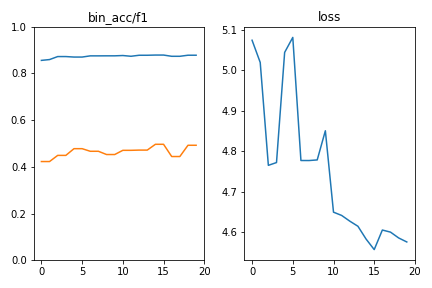
\includegraphics[width=0.8\linewidth]{images/default.png}
		\end{subfigure}%
		\begin{subfigure}{0.5\textwidth}
			\centering
			\caption{More Dense Layers (2)}
			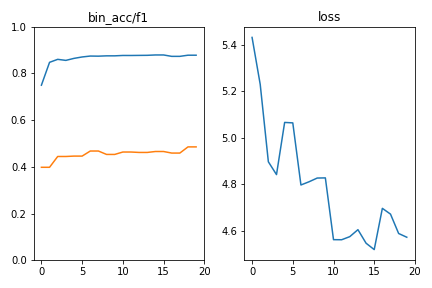
\includegraphics[width=0.8\linewidth]{images/inc_deep_conn_lay.png}
		\end{subfigure}
		\begin{subfigure}{0.5\textwidth}
			\centering
			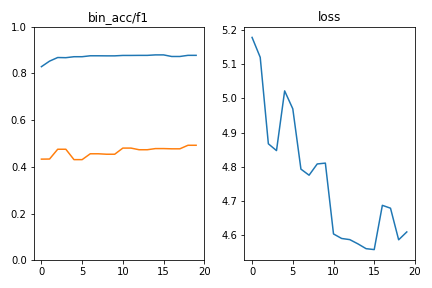
\includegraphics[width=0.8\linewidth]{images/even_more_conv.png}
			\caption{More Convolutional Layers (6)}
		\end{subfigure}%
		\begin{subfigure}{0.5\textwidth}
			\centering
			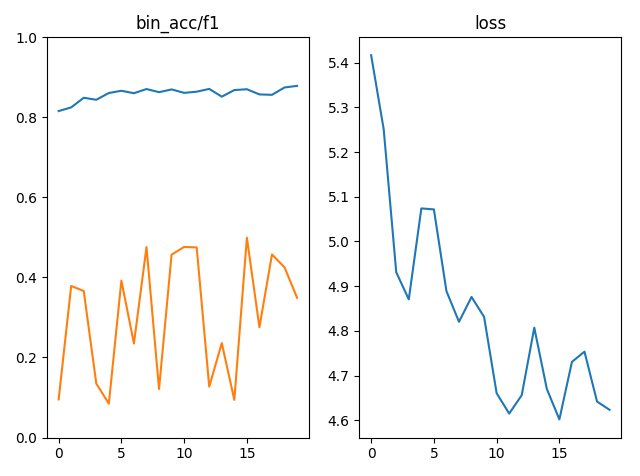
\includegraphics[width=0.8\linewidth]{images/relu_to_tanh.png}
			\caption{\texttt{tanh} (9.2)}
		\end{subfigure}
	\end{figure}
\end{frame}
